% !TeX root = ../main.tex

\chapter{The semi-classical (true) variational approach (WD)}

Starting from the two problems
\begin{center}
  \begin{minipage}{.48\linewidth}
    \centering
    \begin{tikzpicture}
      \draw (0,0) node [left] {$A$}
        to[bend right = 10] (2,-2) node [right] {$B$};
    \end{tikzpicture}
    \[
      \delta \int \d \tau = 0
    \]
  \end{minipage}
  \hspace* \fill
  \begin{minipage}{.48\linewidth}
    \centering
    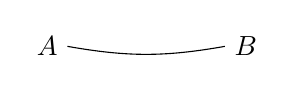
\begin{tikzpicture}
      \draw (0,0) node [left] {$A$}
        to[bend right = 10] (2,0) node [right] {$B$};
    \end{tikzpicture}
    \[
      \delta \int \d l F = 0
    \]
  \end{minipage}
\end{center}
We actually let $\delta \int \d \mathcal L = 0$, i.e., the Euler-Lagrangian EOM.
If it contains the interaction term, then we have the
\emph{Differential-intego-equation}

\section{Variational calculation for free fermions}

\[
  F[n(E)] = \tilde E[n(E)] - TS[n(E)] = \int \d E\phi(E,n)
\]
where $S = -n\ln n - (1 - n)\ln(1 - n)$.
The particle number conservation
\[
  N = \int \d E g(E) n(E), \quad \tilde E = \int \d E E n(E)
\]
We have to minimize the density function
\begin{equation}
  \fdv F{n(E)} \Rightarrow \pdv\phi n = \cdots \Rightarrow
  n^0(E) = \frac1{\upe^{(E-M)/T} + 1}
\end{equation}
also for $\fdv F\mu$.

\subsection{Generic variation around $n^0$}

The energy
\[
  E_0 = \int \frac{\d^ak}{(2\pi)^a} n_k^0 (\epsilon(k))
\]
where $\delta$ expanding some functional (function of functions)
\[
  \delta n_k(\epsilon(k)) = \nu^0(k)
+ \underbrace{\sum_{i = x_i} \pdv n{k_i}
  \bigg|_{n_k^1 \to n^0}}_{\delta(k - k)F,\ \text{The quasi-particle weight}}
  \nu_{k_i}^{(1)} + \frac12 \sum_{i,j} \pdv n{k_i,k_j}
  \underbrace{\nu_{k_ik_j}^{(2)}}_{\pdv n{k_i,k_j}}
\]
To the energy,
\[
  \delta E_0 = \delta \int \frac{\d k}{2\pi} n_k \epsilon_k
= \int \frac{\d k}{2\pi} \epsilon_k \delta n_k
\]
To put $\delta n_k$ into it,
\[
  \fdv En = \fdv*[fun]{\delta E_0 + V(\delta n_k)}n = 0
\]
Now, focus on $T = 0$, then $n_k^{(0)} = \Theta (\epsilon(k) - \mu)$,
$\epsilon_{k_F} - \mu = 0$
\[
  \pdv{n_k^{(0)}}k = \delta(\epsilon(k) - \mu)
  \pdif{k_i} \epsilon \big|_{k\to k_F}
\]
Then, the second derivative
\[
  \pdv{n^{(0)}}{k_i,k_j}
= \ab[\underbrace{\delta (\epsilon - \mu)}_{\delta(k_\bot - k_{F,\bot})}
    \pdif[2]{k_ik_j} \epsilon(k)   \big|_{k\to k_F}
    + \delta'(\epsilon - \mu) \pdif{k_i} \epsilon \pdif{k_j} \big|_{k\to k_F}]
\]
Note that $\delta(k_\bot - k_{F,\bot}) \neq \delta(k - k_r)$, since the shape of
the Fermi surface is arbitrary.
where we can spearate the motion around the Fermi surface into the
parallel and perpendicular terms.
In the simple case single connected Fermi surface
\[
  k_F(\theta) = (k_{r,F}(\theta) \cos\theta, k_{r,F}(\theta) \sin\theta)
\]
where $k_{r,F} (\theta) = k_{r,F_0} + k^0\cos\theta + \cdots$.

Now, we can build the connection between energy and 
\begin{equation}
  \delta E = \int \d \theta \d k_r k_r(\epsilon - \mu)
  (\nu^{(0)} + \delta(k_r - k_{r,F}(\theta)))
  (\pdif{k_r}\epsilon \nu_{k_r} + k_r^{-1} \pdif\theta\epsilon \nu_\theta
  + \frac12 \pdif[2]{k_r} \epsilon \nu_{k,k_r} + \cdots) + 
  \frac12\delta'(\epsilon(k) - \mu) (\qquad)
\end{equation}
where
\[
  \nu_{k_r} = \frac{\nu_{k_x}}{\cos\theta} + \frac{\nu_{k_y}}{\sin\theta}, \quad
  \nu_{k_\theta} = -\frac{\nu_{k_x}}{\sin\theta} + \frac{\nu_{k_y}}{\cos\theta}
\]
where the derivative to the $\delta$-function can be expressed as
\[
  \delta'(\epsilon - \mu)
= \pdif\epsilon \delta(k_r(\epsilon) - k_{r,F}(\epsilon))
= (\pdif\epsilon k_r(\epsilon) - \pdif\epsilon \theta(\theta)
  \pdif\theta k_{r,F}) \delta'(k_r - k_{r,F})
\]
and
\[
  \epsilon(k) \Rightarrow k(\epsilon) = \epsilon^{(-1)}(k)
= [(\pdif{k_r}\epsilon)^{-1} + (\pdif\theta\epsilon)^{-1} \pdif\theta k_{r,F}]
  \delta'(\cdots)
\]
The $\delta E$ can have a compact form
\begin{equation}
  \delta E = \delta E^{(0)}
+ \int\d\theta\d k_r k_r \delta^{(T)}(k_r - k_{r,F})
  [(\epsilon - \mu) \pdif{k_r}F + \pdif{k_r}(\epsilon F)]
\end{equation}
where
\[
F =
  [(\pdif{k_r}\epsilon)^{-1} - (\pdif\theta\epsilon)^{-1} \pdif\theta k_{r,F}]
  \frac12 (\pdif{k_r}\epsilon)^2 \nu_{k_r,k_\theta}z + \cdots +
  (\quad)\nu_{k_r,k_r} + (\quad) \nu_{k_\theta k_\theta}
\]

\subsection{Understanding Fermi Liquid: Particle-hole-pairs (LPHPS)}

Bosonization -- 1D case.

The ``vacuum'' state $\ket|\bm 0>_0$, where $c_k\ket|\bm 0> = 0$, with $k > 0$.
The particle number $N$,
\[:\hat A\hat B\hat C: = ABC - \braket<\bm0|ABC|\bm0>\]
For Bosonic, particle-hole-pair operators
\[
  b_q^\dagger = \frac1{\sqrt{n_q}} \sum_{k=-\infty}^\infty c_{k+q}^\dagger c_k, \quad
  b_q = -\frac\iu{\sqrt{n_q}} \sum c_{k-q}^\dagger c_k
\]
where $q = \frac{2\pi}{L} n_q$, $(b_q^\dagger)^\dagger \to b_q \to b_{-q}^\dagger$.
The particle number
\[
  N_q = b_q^\dagger b_q
\]
If $q > 0$, then without the term $b_{-q}^\dagger$.

The commutator
\[
  [b_q, b_{q'}] = \delta_{q,q'}, \quad
  [b_q^\dagger, b_q'] = \sum\frac1{n1}
  (:c_{k+q-q'}^\dagger c_k - c_{k+q}^\dagger c_{k+q'}:)
= \sum_{k=-\infty}^\infty \frac1{n_q}
  (:c_k^\dagger c_k - c_{k+q}^\dagger c_{k+q}:)
= \delta_{qq'} + \mathcal O(1/k_F)
\]
where $\ket|\bm 0>$ is bosonic ground state
\[
  b_q \ket|\bm N_0> = 0
\]
Look at a typical Fermonic Hamiltonian
\begin{equation}
  \mathcal H = \sum E_p n_p
+ \frac\lambda2 \sum V(q)
  \underbrace{c_{p-q}^\dagger \underbrace{c_{p'+q}^\dagger c_{p'}} c_p}_
  {\frac\lambda2 \sum_{q,k_F,k_F'}V(q)k_{q,k_F}^\dagger b_{q,k_{F'}}}
\end{equation}
The first sum term
\[
  [n_p, b_q^\dagger] = \pm \delta_{p,q} n_q
\]
Then, we obtain the spectral generating algebra
\[
  \sum_{q>0} q b_{q,k_F}^\dagger b_{q,k_F}
+ \frac\lambda2 \sum_{q,k_F,k_F'} b_{q,k_F}' b_{q,k_{F'}}
\equiv \mathcal H_\text{eff}
\]
i.e., the integral equation of $\theta$. The energy
\[
  E(q) \begin{cases}
    \to q/m^*,\\\to \text{Collative hole zero sound}
  \end{cases}
\]
and the matrix form
\[
  \begin{pmatrix}
    q & V(1) & k_fk_{F'}\\
      & \ddots & \ddots \\
    \ddots & & q
  \end{pmatrix}
\]
From $\ket|\bm N_0> \to \ket|\bm\Phi_0>$, $n^0 \to \delta n_p$
jump $Z$ from $Z_1$ to $Z_k$,
\[
  \braket<c^\dagger c^\dagger cc> \to \braket<b_{qk_F}^\dagger b_{qk_{F'}}>
  \propto 1 - Z_k
\]
Identify the \emph{Low energy excitations} (of $\ket|\bm N_0>$).
The interactioin will tend to lower the excited energy.
The interaction will populate the occupy excitations.
If do the canonical
\[
  U\ket|\Phi_0> \Rightarrow (\cdots b^\dagger b^\dagger \cdots) \ket|\bm N_0>
\]